%============================ MAIN DOCUMENT ================================
% define document class
\PassOptionsToPackage{table}{xcolor}
\documentclass[
  a4paper,
  BCOR=15mm,            % Binding correction
  twoside,
% openright,
%  headings=openright,
  bibliography=totoc,   % If enabled add bibliography to TOC
  listof=totoc,         % If enabled add lists to TOC
  monolingual,
% bilingual,
  invert-title,
]{bfhthesis}

\usepackage[french,ngerman,main=english]{babel}  % https://www.namsu.de/Extra/pakete/Babel.html
\LoadBFHModule{listings,terminal,boxes}
%---------------------------------------------------------------------------
% Documents paths
%---------------------------------------------------------------------------
\makeatletter
\def\input@path{{content/}}
%or: \def\input@path{{/path/to/folder/}{/path/to/other/folder/}}
\makeatother
%-----------------  Base packages     --------------------------------------
% Include Packages
\usepackage{amsmath}          % various features to facilitate writing math formulas
\usepackage{amsthm}           % enhanced version of latex's newtheorem
\usepackage{amsfonts}         % set of miscellaneous TeX fonts that augment the standard CM
\usepackage{amssymb}          % mathematical special characters

\usepackage{siunitx}

\usepackage{graphicx}         % integration of images
\usepackage{float}            % floating objects

\usepackage{caption}          % for captions of figures and tables
\usepackage{subcaption}       % for subcaptions in subfigures
\usepackage{cite}             % use bibtex
\usepackage{wrapfig}

\usepackage{exscale}          % mathematical size corresponds to textsize
\usepackage{multirow}         % multirow emables combining rows in tables
\usepackage{multicol}

\usepackage{longtable}

%---------------------------------------------------------------------------
% Graphics paths
%---------------------------------------------------------------------------
\graphicspath{{pictures/}{figures/}}
%---------------------------------------------------------------------------
% Blind text -> for dummy text
%---------------------------------------------------------------------------
\usepackage{blindtext}    
\usepackage{letltxmacro}   
\LetLtxMacro{\blindtextblindtext}{\blindtext}

\RenewDocumentCommand{\blindtext}{O{\value{blindtext}}}{
	\begingroup\color{BFH-Gray}\blindtextblindtext[#1]\endgroup
}
%---------------------------------------------------------------------------
% Glossary Package
%---------------------------------------------------------------------------
% the glossaries package uses makeindex
% if you use TeXnicCenter do the following steps:
%  - Goto "Ausgabeprofile definieren" (ctrl + F7)
%  - Select the profile "LaTeX => PDF"
%  - Add in register "Nachbearbeitung" a new "Postprozessoren" point named Glossar
%  - Select makeindex.exe in the field "Anwendung" ( ..\MiKTeX x.x\miktex\bin\makeindex.exe )
%  - Add this [ -s "%tm.ist" -t "%tmx.glg" -o "%tm.gls" "%tm.glo" ] in the field "Argumente"
%
% for futher informations go to http://ewus.de/tipp-1029.html
%---------------------------------------------------------------------------
\usepackage[nonumberlist]{glossaries-extra}
\makeglossaries
%----------------  Glossary Entries  ---------------------------------------
\newglossaryentry{latex}{
    name=LaTeX,
    description={Ein Textsatzsystem für wissenschaftliche Dokumente}
}

\newglossaryentry{bfh}{
    name=BFH,
    description={Berner Fachhochschule}
}

%----------------  Acronyms  -----------------------------------------------
\newacronym{ai}{AI}{Artificial Intelligence}
\newacronym{ml}{ML}{Machine Learning}
%---------------------------------------------------------------------------
% Makeindex Package
%---------------------------------------------------------------------------
\usepackage{makeidx}
\makeindex
%\usepackage{imakeidx}          % To produce index
%\makeindex[columns=2,intoc]    % Index-Initialisation
%\makeindex[columns=3,columnseprule,columnsep,intoc]
%---------------------------------------------------------------------------
% Hyperref Package (Create links in a pdf)
%---------------------------------------------------------------------------
\usepackage[
	,bookmarks
	,plainpages=false
	,pdfpagelabels
        ,pdfusetitle
	,backref = {false}          % No index backreference
	,colorlinks = {true}        % Color links in a PDF
	,hypertexnames = {true}     % no failures "same page(i)"
	,bookmarksopen = {true}     % opens the bar on the left side
	,bookmarksopenlevel = {0}   % depth of opened bookmarks
	,linkcolor=.
	,filecolor=.
	,urlcolor=.
	,citecolor=.
]{hyperref}
%---------------------------------------------------------------------------

%% %% Customize Footer and Headers in Document
%% \KOMAoptions{headsepline,plainheadsepline,footsepline,plainfootsepline}%
%% \setkomafont{headsepline}{\color{BFH-DarkBlue}}% BFH-DarkBlue required bfhcolors
%% \setkomafont{footsepline}{\color{BFH-DarkBlue}}%
%% \lehead*{lehead} % the * character does replace the header on the first chapter page as well
%% \cehead*{cehead}
%% \rehead*{rehead}
%% \lohead*{lohead}
%% \cohead*{cohead}
%% \rohead*{rohead}

%% \lefoot*{lefoot}
%% \cefoot*{cefoot}
%% \refoot*{refoot}
%% \lofoot*{lofoot}
%% \cofoot*{cofoot}
%% \rofoot*{rofoot}
%---------------------------------------------------------------------------
\begin{document}

%% Snippet do redefine German babel translations -- see FAQ latex.ti.bfh.ch for further information or
%% the package documentation https://www.ctan.org/pkg/translations
%% \redefinetranslation{German}{Advisor}{Dozentin}
%% \redefinetranslation{German}{advisor}{Dozentin} %  just for consistency
%% \redefinetranslation{German}{Author}{Autorin}
%% \redefinetranslation{German}{author}{Autorin} %  just for consistency
%% \redefinetranslation{German}{Co-advisor}{Mitbetreuerin}
%% \redefinetranslation{German}{co-advisor}{Mitbetreuerin} %  just for consistency
%% \redefinetranslation{German}{Expert}{Expertin}
%% \redefinetranslation{German}{expert}{Expertin} %  just for consistency
%% \redefinetranslation{German}{Project partner}{Projektpartnerin}
%% \redefinetranslation{German}{project partner}{Projektpartnerin} %  just for consistency

%------------ START FRONT PART ------------
\frontmatter

\title{Bachelor's Thesis}
\subtitle{Thesis subject}
\author{Anton Muster \and Cindy Example}
\institution{Bern University of Applied Sciences}
\department{Technik und Informatik}
\institute{Mikro- und Medizintechnik}
\version{1.0}
\titlegraphic*{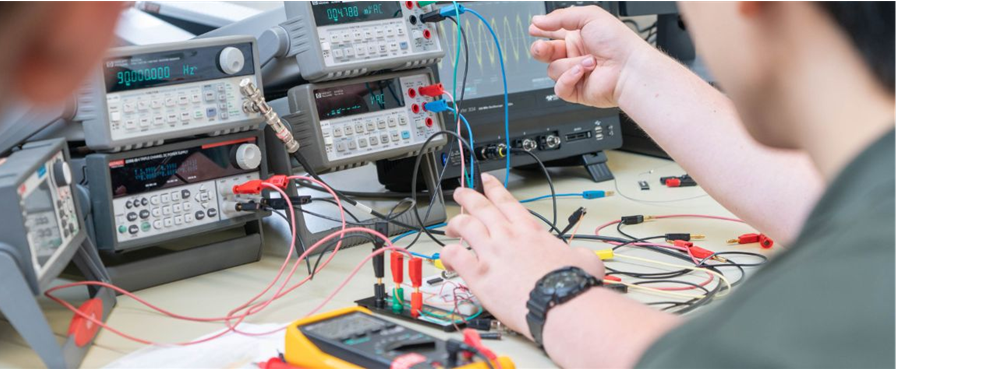
\includegraphics{Bild1.png}}
\advisor{Prof. Dr. Super Smart}
\coadvisor{PhD A. Smart}
\projectpartner{proj partner}
\expert{Some expert}
\degreeprogram{Bachelor of Science in Computer Science}
\setupSignature{
	A. Muster={
\includegraphics[width=.5\linewidth]{sig_muster}},
	C. Example={
\includegraphics[width=.5\linewidth]{sig_example}}
}


%----------------  BFH tile page   -----------------------------------------
\maketitle
%------------ ABSTRACT        ----------------
\addchap{Abstract}
One-paragraph summary of the entire study – typically no more than 250 words in length (and in many cases it is well shorter than that), the Abstract provides an overview of the study.

%------------ TABLEOFCONTENTS ----------------
\tableofcontents

%------------ START MAIN PART ------------
\mainmatter

\chapter{First Thesis Chapter}
\section{Introduction}

What is the topic and why is it worth studying? – the first major section of text in the paper, the Introduction commonly describes the topic under investigation, summarizes or discusses relevant prior research (for related details, please see the Writing Literature Reviews section of this website), identifies unresolved issues that the current research will address, and provides an overview of the research that is to be described in greater detail in the sections to follow.
Das Ziel des Abschnitts «Methoden und Materialien» ist es, dem Leser die Gelegenheit zu bieten, alle Phasen des Versuchs reproduzieren zu können.

\begin{itemize}
    \item[-] Beschreiben Sie Ihre Herangehensweise inklusive Arbeitsaufteilung und den Ablauf des Versuchs. Zitieren Sie dabei jeweils zusätzlich verwendete Ressourcen [8] und referenzieren Sie diese im Literaturverzeichnis.
    \item[-] Listen Sie alle genutzten Geräte [9] und Software [2] und referenzieren Sie jeweils deren Dokumentation im Literaturverzeichnis.
\end{itemize}

\gls{latex} wird oft für wissenschaftliche Arbeiten genutzt. \gls{ai} ist ein Teilbereich von \gls{ml}. Zweite Verwendung von \gls{ai} und \gls{ml}. Test \gls{bfh}.


Hier wird ein Werk zitiert.\cite{EinsteinCoefficientsSpringerLink}

Hie rwird ein weiteres Werk zitiert.\cite{5GrundlagenFur2025}

% ----------------- Bilder -----------------
\begin{figure}[H]
    \centering
    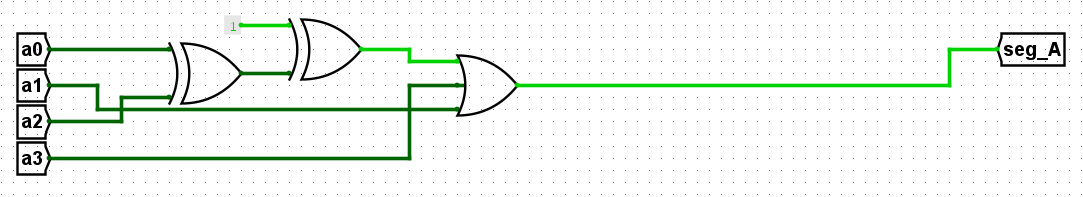
\includegraphics[width=1\textwidth]{segment_A.png}
    \caption{Logikschaltung Segment A}
    \label{fig:segment_A}
\end{figure}

Die Logikschaltung zum Segment A wurde wie in Abbildung~\ref{fig:segment_A} gezeigt aufgebaut.

\begin{figure}[H]
    \centering
    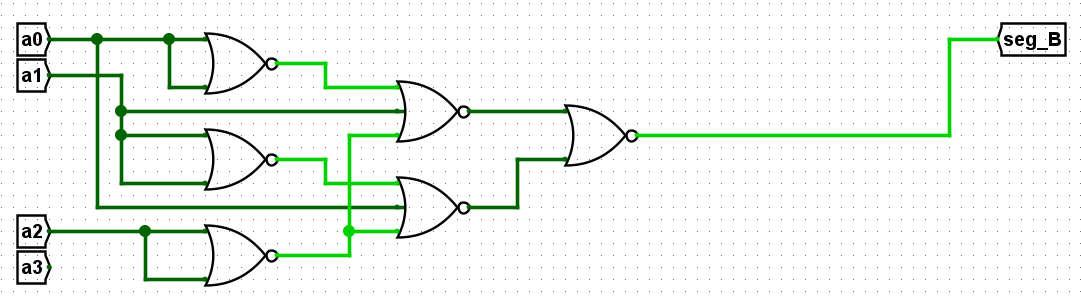
\includegraphics[width=1\textwidth]{segment_B.png}
    \caption{Logikschaltung Segment B}
    \label{fig:segment_B}
\end{figure}

Die Logikschaltung zum Segment B wurde wie in Abbildung~\ref{fig:segment_B} gezeigt aufgebaut.

\begin{figure}[H]
    \centering
    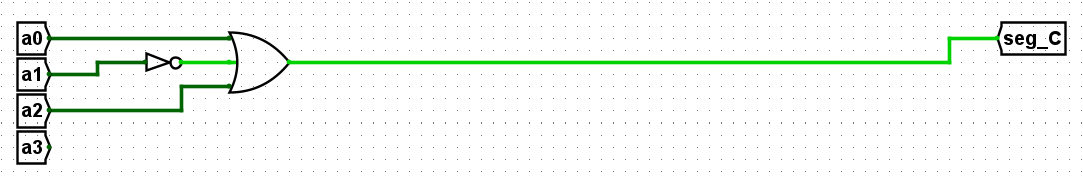
\includegraphics[width=1\textwidth]{segment_C.png}
    \caption{Logikschaltung Segment C}
    \label{fig:segment_C}
\end{figure}

Die Logikschaltung zum Segment C wurde wie in Abbildung~\ref{fig:segment_C} gezeigt aufgebaut.

% ----------------- Tabelle -----------------
\vspace{1em} % Abstand
Nachfolgend die Wahrheitstabelle der Segmente:
\begin{table}[ht]
\centering
\colorlet{BFH-table}{BFH-MediumBlue!10}
\colorlet{BFH-tablehead}{BFH-MediumBlue!50}
\setupBfhTabular
\begin{bfhTabular}{llllllllllll}
Input & a3 & a2 & a1 & a0 & seg\_A & seg\_B & seg\_C & seg\_D & seg\_E & seg\_F & seg\_G \\\hline
\num{0} & \num{0} & \num{0} & \num{0} & \num{0} & \num{1} & \num{1} & \num{1} & \num{1} & \num{1} & \num{1} & \num{0} \\\hline
\num{1} & \num{0} & \num{0} & \num{0} & \num{1} & \num{0} & \num{1} & \num{1} & \num{0} & \num{0} & \num{0} & \num{0} \\\hline
\end{bfhTabular}
\caption{Wahrheitstabelle Siebensegmentanzeige}
\label{tab:truthtable_bcd_to_7segment}
\end{table}
\section{Results}
What did you find? – a section which describes the data that was collected and the results of any statistical tests that were performed.  It may also be prefaced by a description of the analysis procedure that was used. If there were multiple experiments, then each experiment may require a separate Results section.

\chapter{Second Thesis Chapter}
\section{Some \texorpdfstring{\LaTeX}{LaTeX}~Examples}

\blindtext[1]

\subsection{Tabular}

\begin{tabular}[h]{l|l|l}
  \centering
	Measure & Data & Unit \\ \hline
	1      & 2	  & 3  \\
	4      & 5	  & 6
\end{tabular}

% Example for a Table in BFH-Style with a simple Design
\begin{table}[ht]
   \centering
   \begin{bfhTabular}{lll}
      Stadtteil & Anzahl Personen & Ausländische
      Bevölkerung\\\hline
      Innere Stadt & \num{3748} & \SI{17.9}{\percent}\\\hline
      Länggasse-Felsenau & \num{17976} & \SI{17.1}{\percent}\\\hline
      Mattenhof-Weissenbühl & \num{26895} & \SI{22.4}{\percent}\\\hline
      Kirchenfeld-Schlosshalde & \num{23384} & \SI{13.4}{\percent}\\\hline
      Breitenrain-Lorraine & \num{24082} & \SI{19.4}{\percent}
   \end{bfhTabular}
   \caption{Anzahl Personen, ausländischer Bevölkerungsanteil und Arbeitslosenquote pro
	Stadtteil Ende 2005 (Statistikdienste der Stadt Bern, 2006)}
   \label{tab:tab1}
\end{table}

\begin{table}[ht]
   \centering
   \colorlet{BFH-table}{BFH-MediumBlue!10}
   \colorlet{BFH-tablehead}{BFH-MediumBlue!50}
   \begin{bfhTabular}{lll}
      Stadtteil & Anzahl Personen & Ausländische
      Bevölkerung\\\hline
      Innere Stadt & \num{3748} & \SI{17.9}{\percent}\\\hline
      Länggasse-Felsenau & \num{17976} & \SI{17.1}{\percent}\\\hline
      Mattenhof-Weissenbühl & \num{26895} & \SI{22.4}{\percent}\\\hline
      Kirchenfeld-Schlosshalde & \num{23384} & \SI{13.4}{\percent}\\\hline
      Breitenrain-Lorraine & \num{24082} & \SI{19.4}{\percent}
   \end{bfhTabular}
   \caption{Anzahl Personen, ausländischer Bevölkerungsanteil und Arbeitslosenquote pro
	Stadtteil Ende 2005 (Statistikdienste der Stadt Bern, 2006)}
   \label{tab:tab2}
\end{table}

\begin{table}[ht]
   \centering
   \colorlet{BFH-table}{BFH-MediumRed!10}
   \colorlet{BFH-tablehead}{BFH-MediumRed!50}
   \begin{bfhTabular}{lll}
      Stadtteil & Anzahl Personen & Ausländische
      Bevölkerung\\\hline
      Innere Stadt & \num{3748} & \SI{17.9}{\percent}\\\hline
      Länggasse-Felsenau & \num{17976} & \SI{17.1}{\percent}\\\hline
      Mattenhof-Weissenbühl & \num{26895} & \SI{22.4}{\percent}\\\hline
      Kirchenfeld-Schlosshalde & \num{23384} & \SI{13.4}{\percent}\\\hline
      Breitenrain-Lorraine & \num{24082} & \SI{19.4}{\percent}
   \end{bfhTabular}
   \caption{Anzahl Personen, ausländischer Bevölkerungsanteil und Arbeitslosenquote pro
	Stadtteil Ende 2005 (Statistikdienste der Stadt Bern, 2006)}
   \label{tab:tab3}
\end{table}


\begin{description}
\item[More about Tables] Further information about tables : \url{https://www.latex-tutorial.com/tutorials/tables/}
\item[Long Tables] Further information about long tables : \url{https://www.overleaf.com/learn/latex/tables}
\end{description}


\begin{longtable}{|l|l|l|}
\caption{A sample long table} \label{tab:long} \\


\hline \multicolumn{1}{|c|}{\textbf{First column}} & \multicolumn{1}{c|}{\textbf{Second column}} & \multicolumn{1}{c|}{\textbf{Third column}} \\ \hline 
\endfirsthead

\multicolumn{3}{c}%
{{\tablename\ \thetable{}: \hfill $...$~continued from previous page}} \\
\hline \multicolumn{1}{|c|}{\textbf{First column}} & \multicolumn{1}{c|}{\textbf{Second column}} & \multicolumn{1}{c|}{\textbf{Third column}} \\ \hline 
\endhead

\hline \multicolumn{3}{|r|}{{Continued on next page$...$}} \\ \hline
\endfoot

\hline \hline
\endlastfoot
\centering

One & abcdef ghjijklmn & 123.456778 \\
One & abcdef ghjijklmn & 123.456778 \\
One & abcdef ghjijklmn & 123.456778 \\
One & abcdef ghjijklmn & 123.456778 \\
One & abcdef ghjijklmn & 123.456778 \\
One & abcdef ghjijklmn & 123.456778 \\
One & abcdef ghjijklmn & 123.456778 \\
One & abcdef ghjijklmn & 123.456778 \\
One & abcdef ghjijklmn & 123.456778 \\
One & abcdef ghjijklmn & 123.456778 \\
One & abcdef ghjijklmn & 123.456778 \\
One & abcdef ghjijklmn & 123.456778 \\
One & abcdef ghjijklmn & 123.456778 \\
One & abcdef ghjijklmn & 123.456778 \\
One & abcdef ghjijklmn & 123.456778 \\
One & abcdef ghjijklmn & 123.456778 \\
One & abcdef ghjijklmn & 123.456778 \\
One & abcdef ghjijklmn & 123.456778 \\
One & abcdef ghjijklmn & 123.456778 \\
One & abcdef ghjijklmn & 123.456778 \\
One & abcdef ghjijklmn & 123.456778 \\
One & abcdef ghjijklmn & 123.456778 \\
One & abcdef ghjijklmn & 123.456778 \\
One & abcdef ghjijklmn & 123.456778 \\
One & abcdef ghjijklmn & 123.456778 \\
One & abcdef ghjijklmn & 123.456778 \\
One & abcdef ghjijklmn & 123.456778 \\
One & abcdef ghjijklmn & 123.456778 \\
One & abcdef ghjijklmn & 123.456778 \\
One & abcdef ghjijklmn & 123.456778 \\
One & abcdef ghjijklmn & 123.456778 \\
One & abcdef ghjijklmn & 123.456778 \\
One & abcdef ghjijklmn & 123.456778 \\
One & abcdef ghjijklmn & 123.456778 \\
One & abcdef ghjijklmn & 123.456778 \\
One & abcdef ghjijklmn & 123.456778 \\
One & abcdef ghjijklmn & 123.456778 \\
One & abcdef ghjijklmn & 123.456778 \\
One & abcdef ghjijklmn & 123.456778 \\
One & abcdef ghjijklmn & 123.456778 \\
One & abcdef ghjijklmn & 123.456778 \\
One & abcdef ghjijklmn & 123.456778 \\
One & abcdef ghjijklmn & 123.456778 \\
One & abcdef ghjijklmn & 123.456778 \\
One & abcdef ghjijklmn & 123.456778 \\
One & abcdef ghjijklmn & 123.456778 \\
One & abcdef ghjijklmn & 123.456778 \\
One & abcdef ghjijklmn & 123.456778 \\
One & abcdef ghjijklmn & 123.456778 \\
One & abcdef ghjijklmn & 123.456778 \\
One & abcdef ghjijklmn & 123.456778 \\
One & abcdef ghjijklmn & 123.456778 \\
One & abcdef ghjijklmn & 123.456778 \\
One & abcdef ghjijklmn & 123.456778 \\
One & abcdef ghjijklmn & 123.456778 \\
One & abcdef ghjijklmn & 123.456778 \\
One & abcdef ghjijklmn & 123.456778 \\
One & abcdef ghjijklmn & 123.456778 \\
One & abcdef ghjijklmn & 123.456778 \\
One & abcdef ghjijklmn & 123.456778 \\
One & abcdef ghjijklmn & 123.456778 \\
One & abcdef ghjijklmn & 123.456778 \\
One & abcdef ghjijklmn & 123.456778 \\
One & abcdef ghjijklmn & 123.456778 \\
One & abcdef ghjijklmn & 123.456778 \\
One & abcdef ghjijklmn & 123.456778 \\
One & abcdef ghjijklmn & 123.456778 \\
One & abcdef ghjijklmn & 123.456778 \\
One & abcdef ghjijklmn & 123.456778 \\
One & abcdef ghjijklmn & 123.456778 \\
One & abcdef ghjijklmn & 123.456778 \\
One & abcdef ghjijklmn & 123.456778 \\
One & abcdef ghjijklmn & 123.456778 \\
One & abcdef ghjijklmn & 123.456778 \\
One & abcdef ghjijklmn & 123.456778 \\
\end{longtable}
 

\subsection{Math}
%% Mathematical equations
\begin{align}
\left(\begin{array}{r}
\dot{x_{1}} \\                                              
\dot{x_{2}} \\ 
\dot{x_{3}} \\                                 
\end{array}\right) =
\left[\begin{array}{rrr}
0 & 1 & 0 \\                                              
0 & -\frac{b_{f}}{J} & \frac{K_{m}}{J} \\
0 & -\frac{K_{g}}{L} & \frac{R}{L} \\                                      
\end{array}\right]
\left(\begin{array}{r}
x_{1} \\                                              
x_{2} \\ 
x_{3} \\                                 
\end{array}\right) +
\left[\begin{array}{rr}
0 & 0 \\                                              
-\frac{1}{J} & 0 \\ 
0 & \frac{1}{L} \\                                 
\end{array}\right]
\left(\begin{array}{r}
t_{L} \\                                              
v_{a} \\                                 
\end{array}\right)
\end{align}

\subsection{Include pictures}

\begin{figure}[H]
  \centering
  
\includegraphics[width=.8\textwidth]{placeholder}
  \caption{Some meaningful caption}
  \label{fig:placeholder:1}
\end{figure}


\begin{figure}[h!]
  \centering
  \begin{minipage}{.4\textwidth}
  	\centering
	
\includegraphics[width=\textwidth]{placeholder}
	\caption{PLACEHOLDER}
	\label{fig:placeholder:2}
  \end{minipage}
  \hspace{1em}
  \begin{minipage}{.4\textwidth}
	\centering
	
\includegraphics[width=\textwidth]{placeholder}
	\caption{PLACEHOLDER}
	\label{fig:placeholder:3}
  \end{minipage}%
\end{figure}


%% Source code is stored in the listings folder and will be included from there using its relative path.
\subsection{Code Example}

{
  \thicklines
% \thinlines
\lstinputlisting[style=bfh-c,language=C,caption={My very first C program.},label={lst:hello}]{listings/expl_hello.c}
}
I developed this very nice application writing "Hello World" to my terminal.
The implementation is shown in listing~\ref{lst:hello}.


%% Examples holding dummy content
\subsection{Draw boxes}
\begin{bfhBox}[BFH-DarkPurple]{Purple}
	Note\\
\end{bfhBox}

\blindtext[1]

\begin{bfhBox}[BFH-MediumBlue]{Blue}
	Note\\
\end{bfhBox}

\blindtext[1]

\begin{bfhBox}[BFH-DarkRed]{Red}
	Note\\
\end{bfhBox}

\blindtext[2]

\begin{bfhAlertBox}
  An alert box.
\end{bfhAlertBox}

\begin{bfhWarnBox}
  A warning box.
\end{bfhWarnBox}

\begin{bfhNoteBox}
  A note box.
\end{bfhNoteBox}

\begin{bfhRecycleBox}
  A recycle box.
\end{bfhRecycleBox}


\begin{bfhBox}{No color set}
	Some BFH box without color option set. Using default.\\
\end{bfhBox}


\blindtext[3]


\subsection{Some Item-list}
Sometimes you explain this and that using a bullet points.
This can be done in \LaTeX\ using an item list in a item environment.

\begin{itemize}
\item My first item
\item The second
\item $\cdots$
\item $\cdots$
\end{itemize}

It is also possible to nest such environment and/or enumerate.
\begin{itemize}
\item My first item
\begin{enumerate}
\item My first enumerated item
\item The second
\item $\cdots$
\end{enumerate}
\item The second
\begin{enumerate}
\item An other enumerated item
\item $\cdots$
\item $\cdots$
\end{enumerate}
\end{itemize}


\subsection{Multi column environment}
Split a part of a document in multiple columns is not so easy with WYSIWYG tools.
Whit multicols \LaTeX\ package$\cdots$ well you may know.

\begin{multicols}{3}
\begin{itemize}
\item My first item
\item The second
\item $\cdots$
\item $\cdots$
\end{itemize}
\begin{itemize}
\item My first item
\item The second
\item $\cdots$
\item $\cdots$
\end{itemize}
\begin{itemize}
\item My first item
\item The second
\item $\cdots$
\item $\cdots$
\end{itemize}
\end{multicols}


\blindtext[1]

\begin{multicols}{2}
  \blindtext[1]
\end{multicols}

\begin{multicols}{3}
  \blindtext[1]
\end{multicols}

\begin{multicols}{2}
  \blindtext[1]
\end{multicols}


\begin{multicols}{3}
\begin{itemize}
\item My first item
\item The second
\item $\cdots$
\item $\cdots$
\end{itemize}
\blindtext[1]
\columnbreak
\begin{itemize}
\item My first item
\item The second
\item $\cdots$
\item $\cdots$
\end{itemize}
\end{multicols}

%% forced page break
\newpage

\subsection{Use Figures}

\begin{figure}[h!]
  \centering
  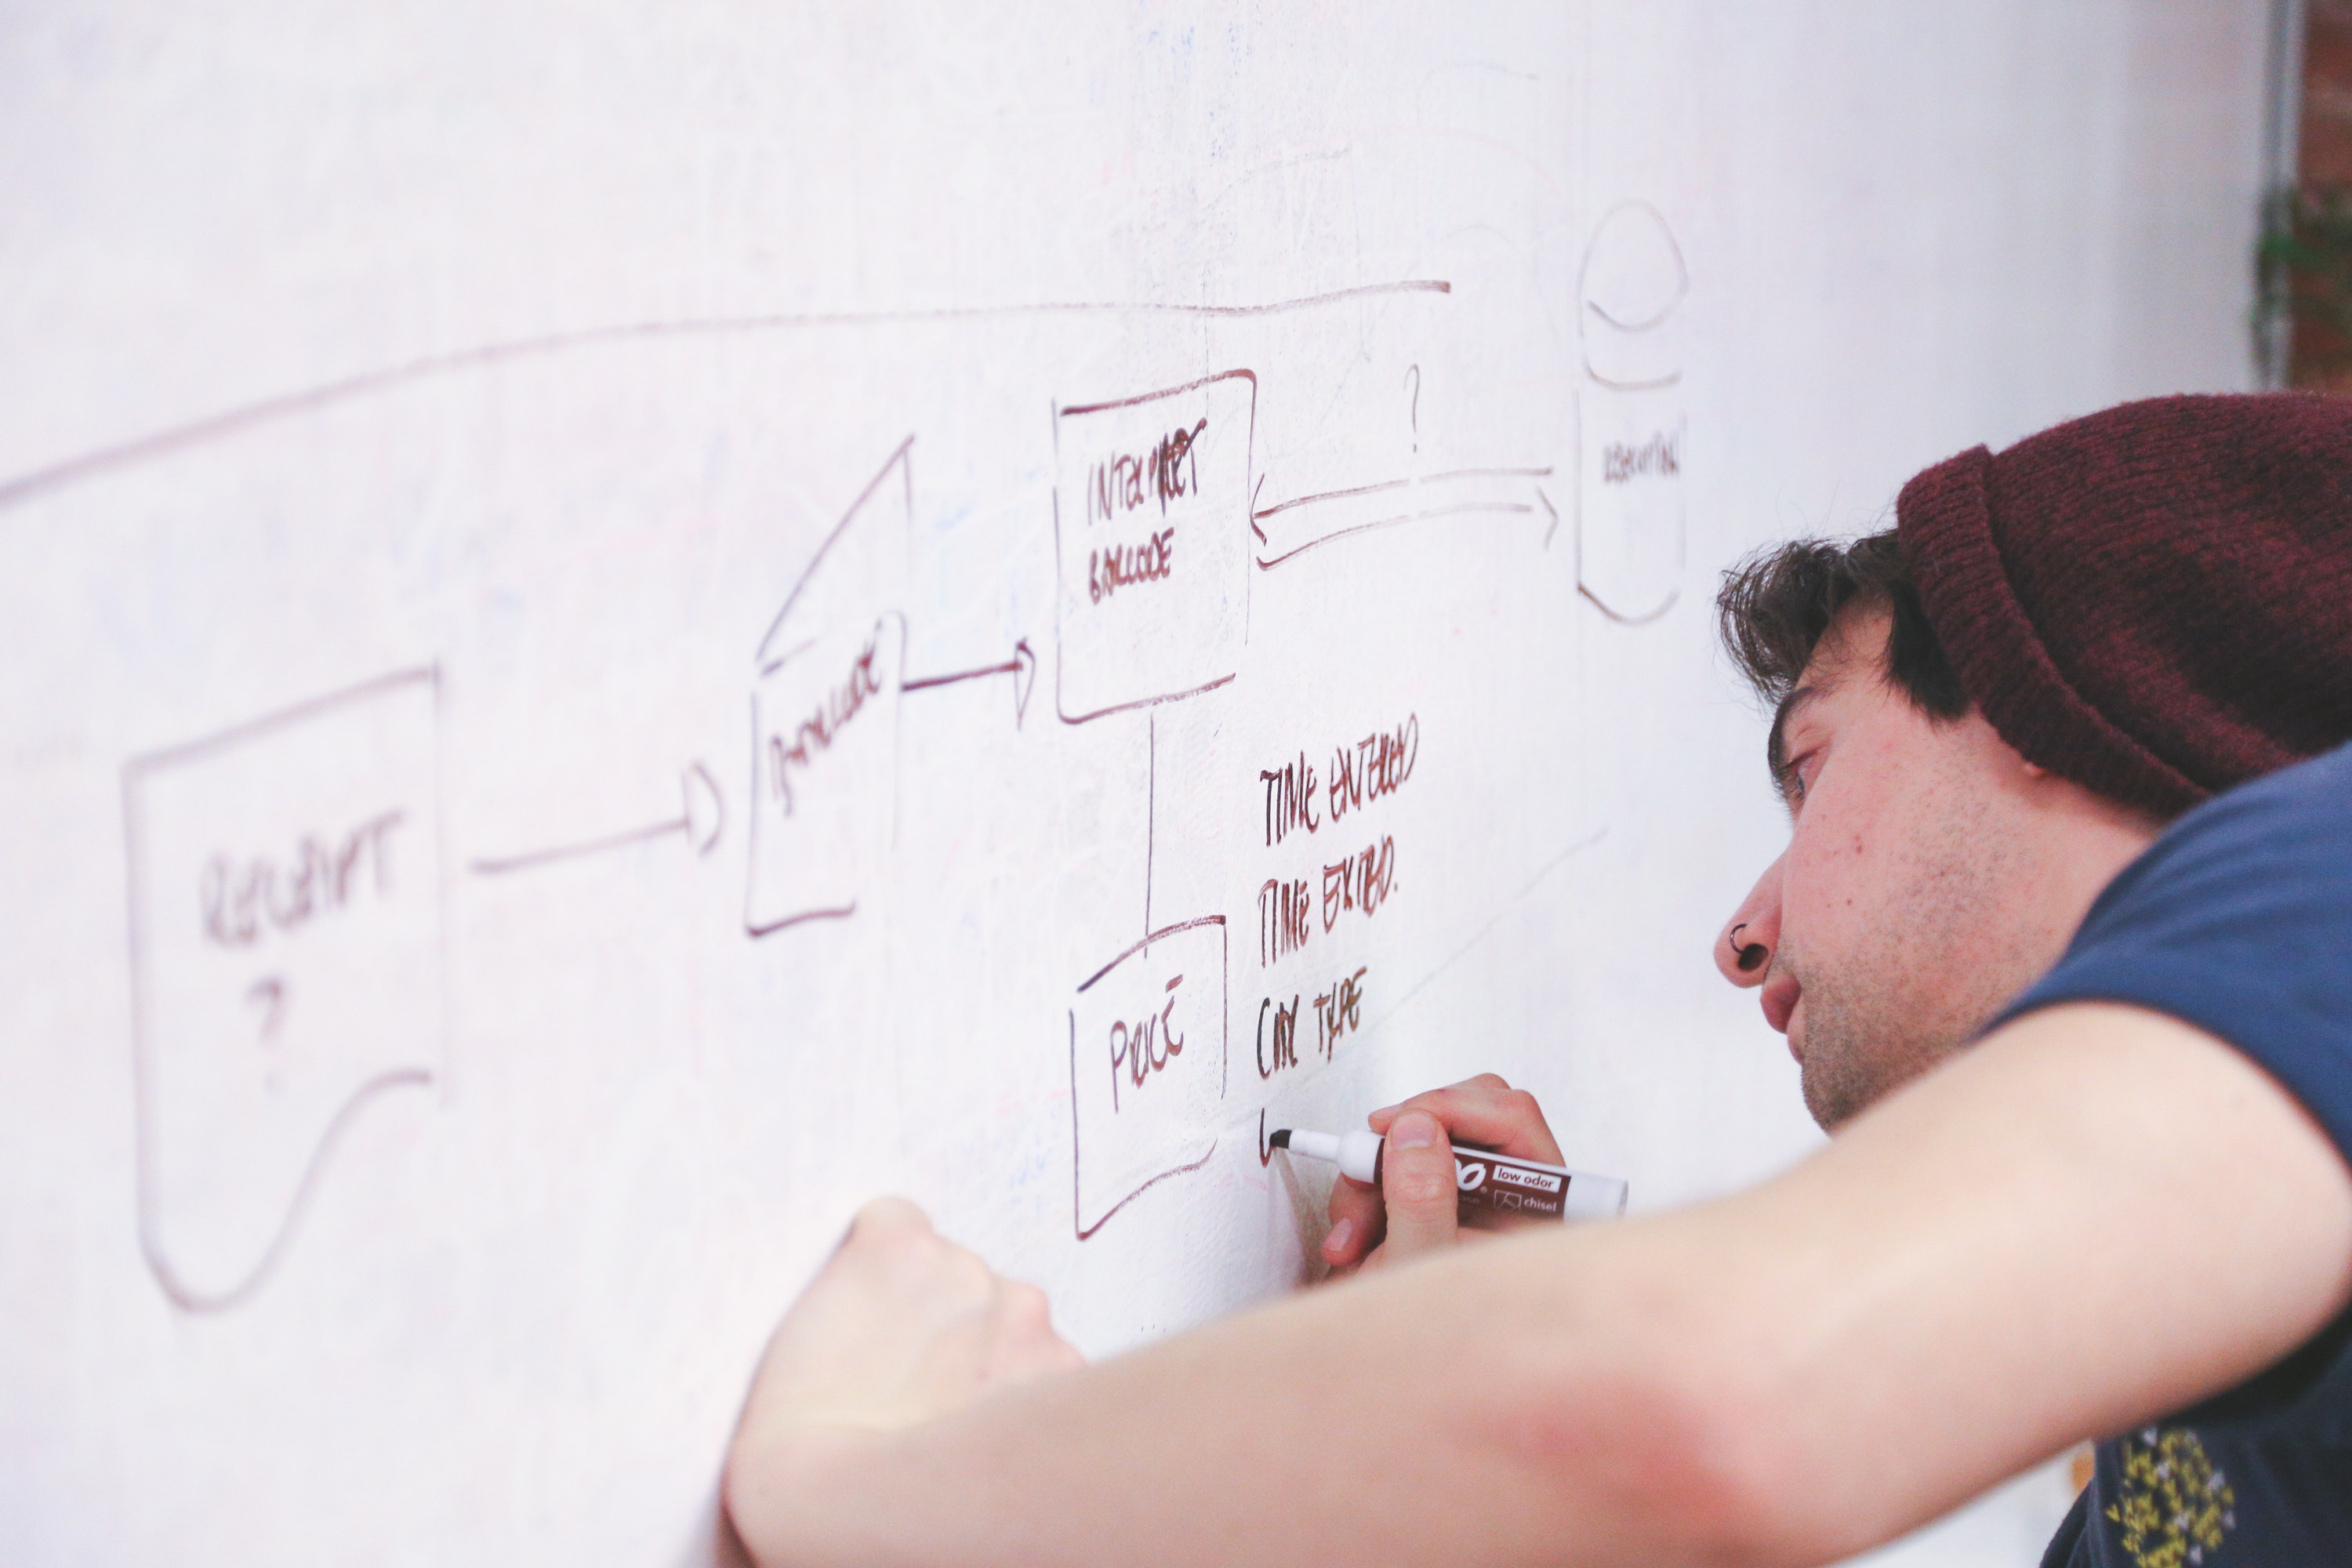
\includegraphics[width=.8\textwidth]{bg-masthead}
  \caption{An example of including a PDF figure.}
  \label{fig:expl_master}
\end{figure}

\begin{figure}[h!]
  \centering
  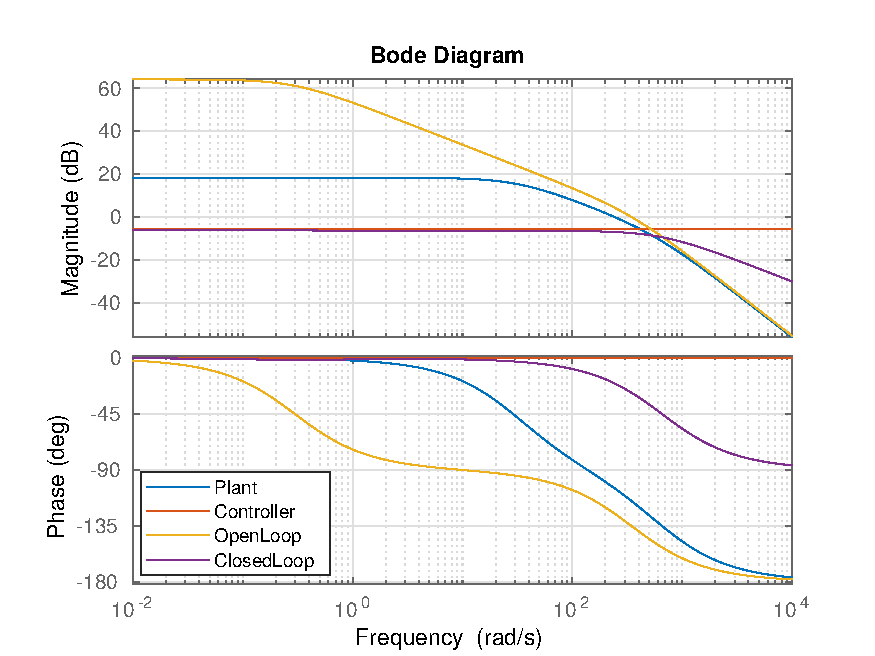
\includegraphics[width=.8\textwidth]{expl_bode}
  \caption{An example of including a PDF figure.}
  \label{fig:expl_bode}
\end{figure}
\clearpage

\subsubsection{Use Subfigures}
These subfigures requires the package \texttt{subcaption}.

\begin{figure}[h!]
     \centering
     \begin{subfigure}[b]{0.3\textwidth}
         \centering
         
\includegraphics[width=\textwidth]{placeholder}
         \caption{$y=x$}
         \label{fig:y equals x}
     \end{subfigure}
     \hfill
     \begin{subfigure}[b]{0.3\textwidth}
         \centering
         
\includegraphics[width=\textwidth]{placeholder}
         \caption{$y=3sinx$}
         \label{fig:three sin x}
     \end{subfigure}
     \hfill
     \begin{subfigure}[b]{0.3\textwidth}
         \centering
         
\includegraphics[width=\textwidth]{placeholder}
         \caption{$y=5/x$}
         \label{fig:five over x}
     \end{subfigure}
        \caption{Three simple graphs}
        \label{fig:three graphs}
\end{figure}


\section{Example Text With Indices}
In this example, several keywords\index{keywords} will be used 
which are important and deserve to appear in the Index\index{Index}.

Terms like generate\index{generate} and some\index{others} will 
also show up.

% \section{Example Text With Glossary}
% This \Gls{zynq} introduction summary has been written for bachelor students due to the introduction workshop in the ``Embedded Systems'' course at Bern University of Applied Sciences. The topic \Gls{soc} is introduced by using Xilinx' \Gls{apsoc} platform \Gls{zynq}. The subsequent summery is a brief introduction only. It is based on several tutorials in the field of \Gls{soc} such as the \Gls{zbook} or Xilinx' \Gls{apsoc} manual. We think the script provides a good introduction and helps getting the overall picture of the \Gls{soc} basics. In addition we reference to our wiki tutorials that provide lots of information on how to get started with the \Gls{zboard}.\\

% Hey folks let's do an \Gls{asic} design and develop some awesome \Gls{rtos}! Yea \Gls{arm} is nice but we can do better, can we?

% \section{Example Text With Citations}
%% Text with citations

% This document is an example of \Gls{BibTeX} using in bibliography management. Three items 
% are cited: The \LaTeX\ Companion book \cite{latexcompanion}, the Einstein
% journal paper \cite{einstein}, and the Donald Knuth's website \cite{knuthwebsite}. 
% The \LaTeX\ related items are \cite{latexcompanion,knuthwebsite}.
Ziel des Abschnitts Diskussion ist es die Ergebnisse des Versuchs zusammenzufassen und zu reflektieren.
–	Erreichte Funktionalität und verbleibende Probleme
–	Fazit und Reflexion

%------------ Authorship declaration translated to main language ------------
\declarationOfAuthorship

%----------- Bibliography ----------------
\clearpage
\bibliographystyle{unsrt}
\bibliography{project}      % the project.bib file gets loaded

%------------ List of Figures ------------
\listoffigures
 
%------------ List of Tables -------------
\listoftables
 
%------------ List of Listings -----------
\lstlistoflistings 
 
%------------ Glossary -------------------
\printglossary

%------------ Index ----------------------
\clearpage
\printindex
%------------ Appendix ----------------	
\appendix
\chapter{First Appendix Chapter}

\end{document}
